% !TeX root=main.tex

\chapter{پیش‌زمینه}
\thispagestyle{empty}

\section{نمونه تقابلی و آموزش تقابلی}
نمونه تقابلی
\LTRfootnote{Adversarial Example/Image}
 یک نسخه دستکاری شده است از یک نمونه، برای مثال تصویر است که عمدا و آگاهانه آشفته و دستکاری شده است تا شبکه را به اشتباه بیندازد.
\\
این نمونه‌ها با تغییر‌های جزئی تقابلی 
\LTRfootnote{Adversarial Perturbation}
در تصویر اصلی به وجود می‌آیند و در حالی که برای انسان‌ها قابل تشخیص نیستند و مشابه
\LTRfootnote{Quasi-imperceptible/Imperceptible}
به نظر می‌رسند، برای شبکه‌ها به شکلی کاملا متفاوت به نظر می‌رسد.
\\
آموزش تقابلی 
\LTRfootnote{Adversarial Training}
نیز به معنی استفاده از نمونه‌های تقابلی در کنار نمونه‌های تمیز و دست نخورده برای آموزش مدل‌های یادگیری عمیق است.

\section{دسته‌بندی انواع حملات تقابلی}
حمله‌های تقابلی
\LTRfootnote{Adversarial Attacks}
در دسته‌بندی های مختلفی مانند حمله هدفمند
\LTRfootnote{Targeted Attack}
و بدون هدف
\LTRfootnote{Untargeted Attack}
، حمله جامع
\LTRfootnote{Universal Attack}
و وابسته به داده
\LTRfootnote{Data Dependent Attack}
، حمله دستکاری
\LTRfootnote{Perturbation}
و جایگذاری
\LTRfootnote{Replacement}
، حمله جعبه سیاه
\LTRfootnote{Black-Box Attack}
، حمله جعبه نیمه‌سفید
\LTRfootnote{Semi-White-Box Attack}
و جعبه سفید
\LTRfootnote{White-Box Attack}
طبقه بندی می‌شوند.

\subsection{حمله‌ جعبه سفید}
در این نوع حمله‌ها این طور در نظر گرفته می‌شود که دانش و اطلاع کامل بر مدل هدف، مقدار‌های پارامتر‌های مدل، معماری، روش آموزش و در برخی موراد داده‌های آموزش در اختیار است.
\subsection{حمله جعبه سیاه}
در حمله‌های جعبه سیاه به یک مدل هدف در مرحله آزمایش، نمونه‌های تقابلی‌ای که بدون دانش از مدل ساخته شده‌اند، داده می‌شوند. در برخی مورد‌ها این طور فرض می‌شود که حمله‌کننده دانش کم و محدودی از مدل به طور مثال روند آموزش و یا معماری آن را دارد ولی قطعا درباره پارامتر‌های مدل چیزی نمی‌داند. 
\subsection{حمله جعبه نیمه‌سفید}
در این نوع حمله که بسیار شبیه به حمله‌های جعبه سیاه و همچین جعبه سفید استاست، با این فرق که هر دانش و اطلاعات دیگری درباره مدل هدف در حمله استفاده می‌شود. به طور مثال می‌تواند احتمال‌هایی که از پیش‌بینی شبکه بدست می‌آید را داشته باشد در حالی که در حمله جعبه سیاه ممکن از تنها پیش‌بینی نهایی یا به عبارت دیگر کلاس پیش‌بینی شده را بداند.
\\
لازم به ذکر است که حمله‌های جعبه سفید بسیار قوی‌تر هستند و بنابراین اگر مدلی بتواند در مقابل این نوع حمله‌ها مقاوم باشد، به طور مشابه می‌تواند در برابر حمله‌های جعبه سیاه و جعبه نیمه سفید مقاوم باشد.


\section{شبکه مولد تقابلی}
شبکه مولد تقابلی یا شبکه زایای دشمن‌گونه
\LTRfootnote{Generative Adversarial Network} \cite{Goodfellow2014GenerativeAN}
، که به اختصار GAN نیز گفته می‌شود، دارای دو بخش اصلی است به نام‌های مولد 
\LTRfootnote{Generator}
و تمییزدهنده
\LTRfootnote{Discriminator}
است. این دو شبکه عصبی عملکردی برضد و برخلاف یکدیگر دارند. این دو شبکه در یک بازی مجموع-صفر
\LTRfootnote{Zero-Sum Game}
با هم به رقابت می‌پردازند.
\\
این شبکه در اصل به عنوان یک مدل مولد
\LTRfootnote{Generative Model}
  برای یادگیری بی‌نظارت 
\LTRfootnote{Unsupervised Learning}
ارائه شده بود ولی شبکه‌های مولد تقابلی برای یادگیری نیمه‌نظارتی
\LTRfootnote{Semi-Supervised Learning}
، یادگیری نظارت‌شده
\LTRfootnote{Supervised Learning}
و یادگیری تقویتی
\LTRfootnote{Reinforcement Learning}
نیز کاربردی اثبات شده‌اند.

\subsection{مولد}
مولد یا تولید کننده، یک نویزی که اغلب به صورت گوسی
\LTRfootnote{Gaussian}
 یا یکنواخت 
\LTRfootnote{Uniform}
 را به عنوان ورودی خود می‌گیرد و سپس تصویر بسیار نویزداری از دیتای ورودی را به وجود می‌آورد.
\\
هدف اصلی مولد این است که تصویر‌های تولید شده تا جای ممکن به تصویر‌های حقیقی و طبیعی مجموعه‌ی داده شباهت داشته باشد.
\\
مولد از نویز‌های تصادفی، تصویر‌هایی با همان ابعاد تصویر‌های مجموعه داده به وجود می‌آورد.

\subsection{تمییز‌دهنده}
تمیز دهنده، جداساز، تفکیک کننده یا تشخیص دهنده یک تصویر را به عنوان ورودی می‌گیرد و وظیفه آن تشخیص تصویر‌های حقیقی (تصویر‌های مجموعه داده) از تصاویر جعلی توسط مولد است.
\\
تمییزدهنده اگر تصویر را طبیعی تشخیص دهد در خروجی مقداری نزدیک به ۰ و اگر تصویر را غیرطبیعی تشخیص دهد مقداری نزدیک به ۱ را می‌دهد.

\subsection{نحوه عملکرد شبکه}
در شبکه مولد تقابلی، هدف این است که مولد بتواند تصویری را به وجود بیاورد که به اندازه‌ی تصویر‌های حقیقی، طبیعی جلوه کنند. به طوری که این تصویر‌ها هم کامپیوتر و هم انسان را بتوانند فریب دهند.
\\
همان طور که در شکل 
\ref{ganArch}
دیده می‌شود، تصویری‌های تولید شده توسط مولد و تصویر‌های مجموعه داده به تمییزدهنده‌ی داده می‌شوند. مولد نیز آموزش می‌بیند که تصویر‌هایی طبیعی‌تر و فریبنده‌تر تولید کند و سپس پس از محاسبه گرادیان‌ها، از این مقادیر برای به روزرسانی پارامترهای هر شبکه استفاده می‌شود.
\begin{figure}[H]
	\center{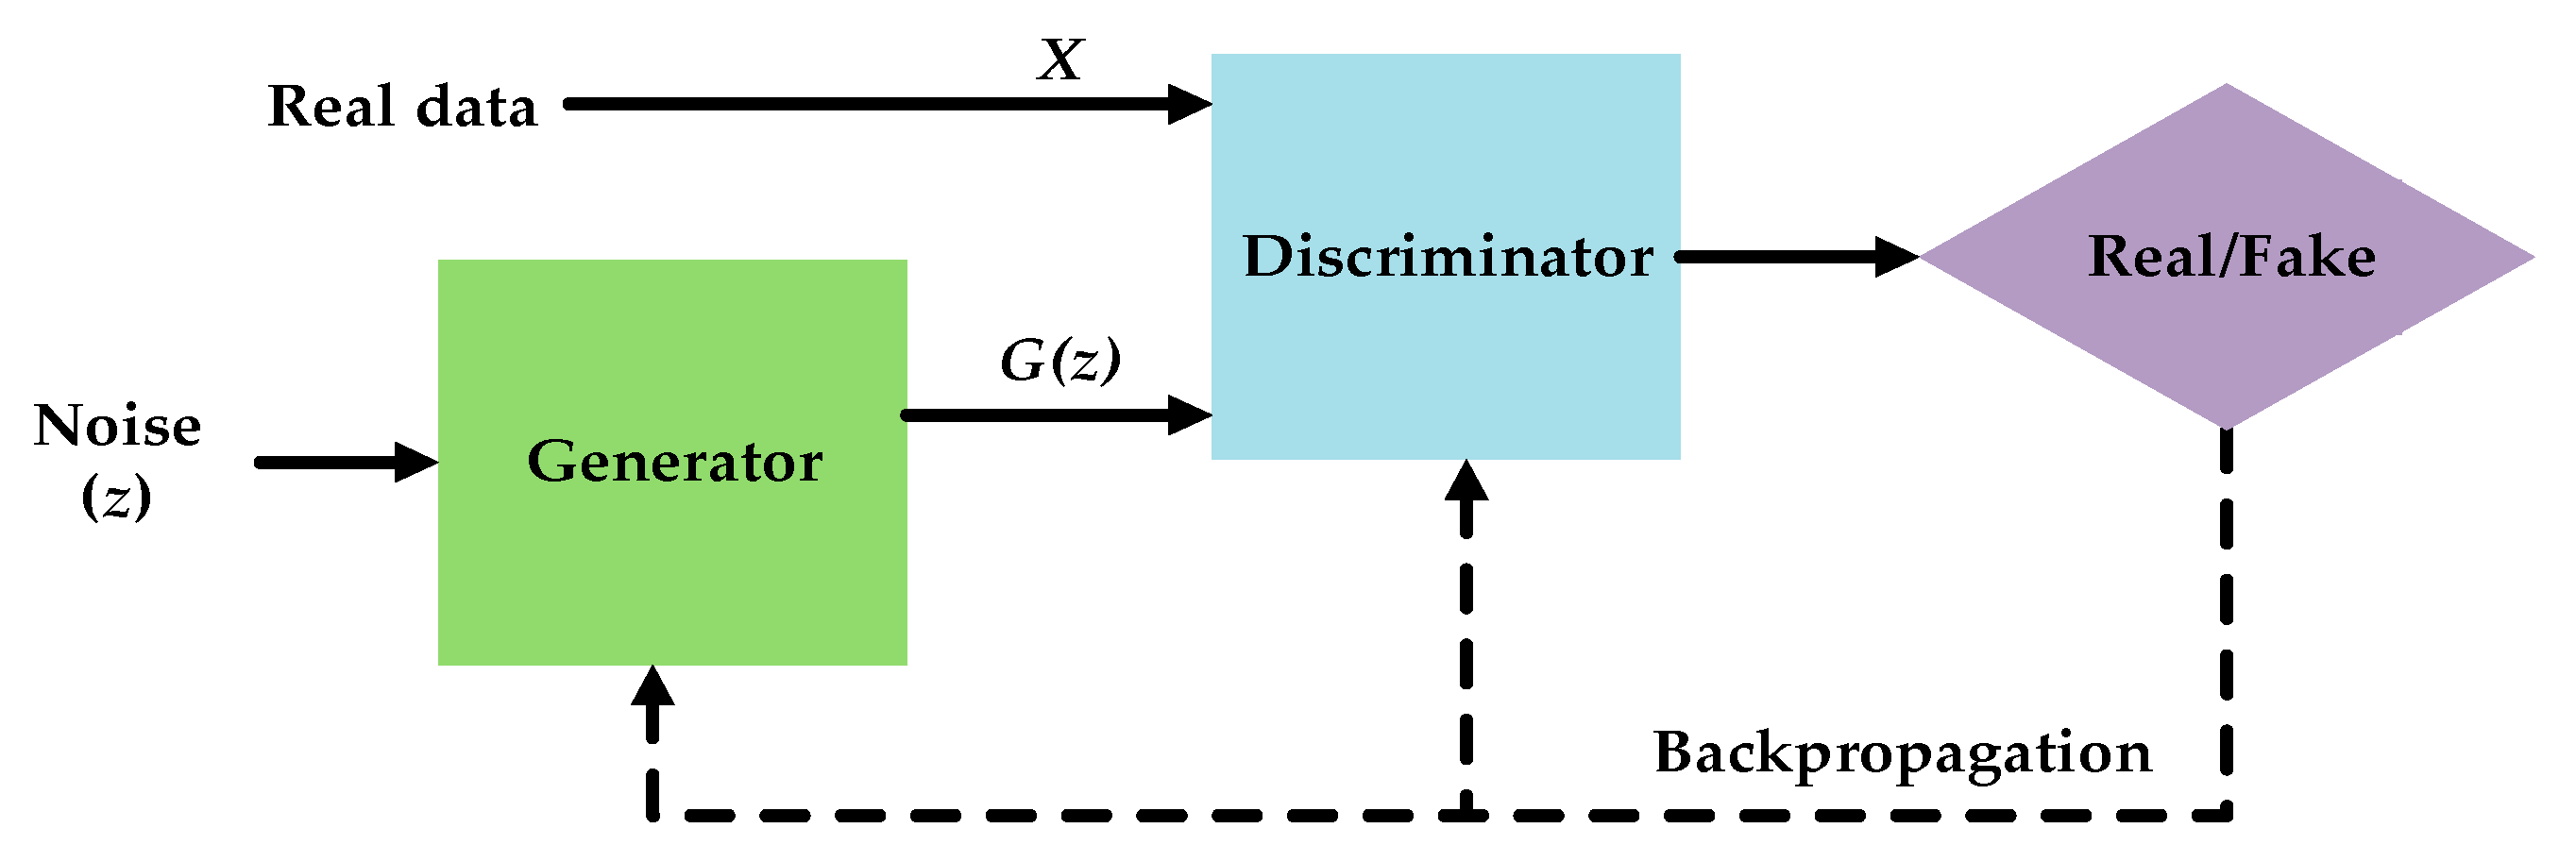
\includegraphics[width=\linewidth]{images/ganArch.PNG}}
	\caption{ساختار یک شبکه مولد تقابلی
		\href{https://bytes860770954.wordpress.com/2020/08/22/what-are-generative-adversarial-networks-gans/}{منبع}}
	\label{ganArch}
\end{figure}

در شکل
\ref{ganlab}
نیز تصویر‌سازی‌ای از روند تعامل و آموزش شبکه مولد تقابلی، که در
 \href{https://poloclub.github.io/ganlab/}{این لینک} 
قابل دسترسی است، آورده شده است .
\begin{figure}[H]
	\center{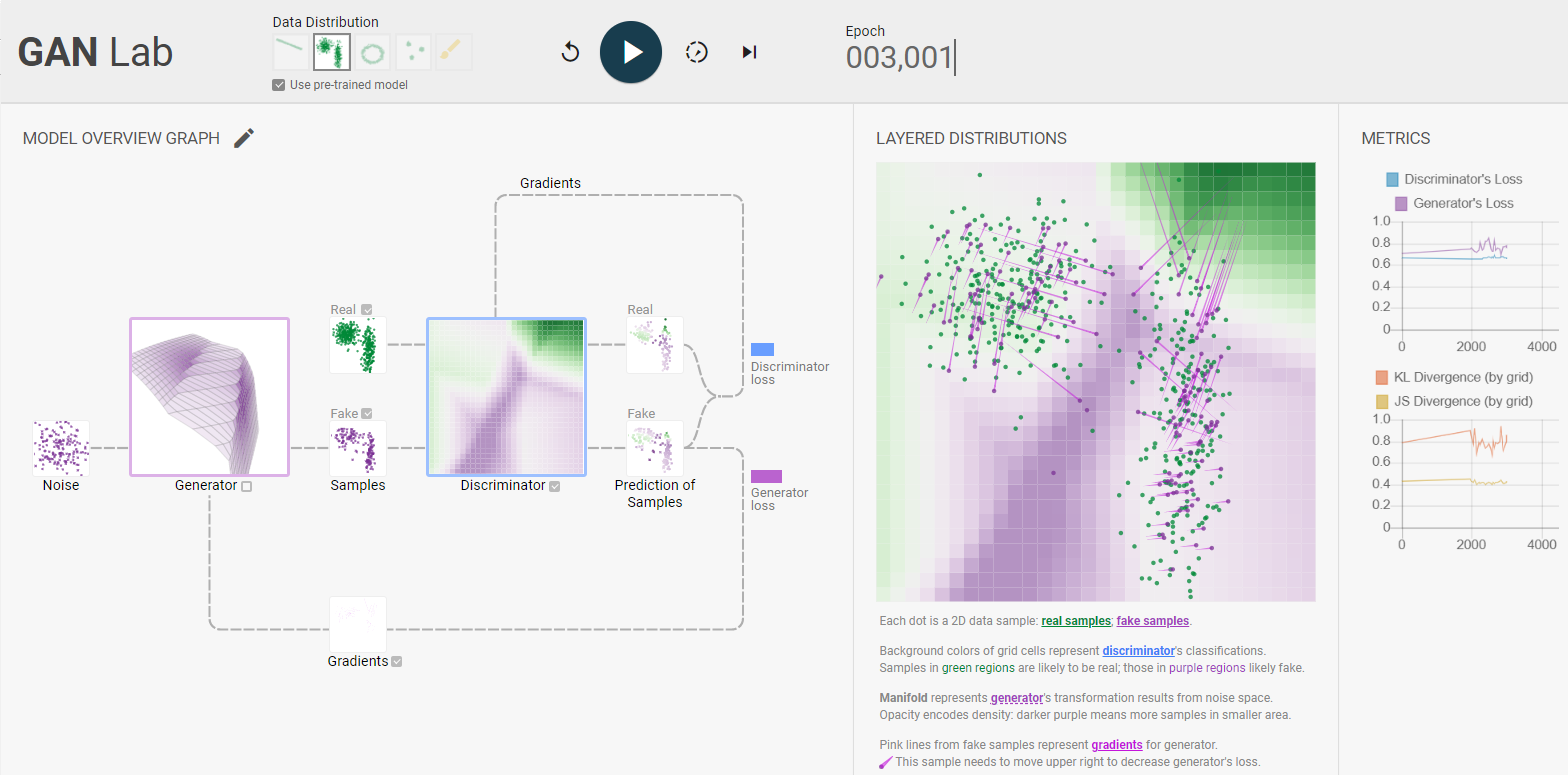
\includegraphics[width=\linewidth]{images/ganlab.PNG}}
	\caption{تصویرسازی روند عملکرد یک شبکه مولد تقابلی}
	\label{ganlab}
\end{figure}
